\section{Part 1}

\subsection{Converting given formula \texttt{F} to 3COL graph}

As the first letter of my first name begins with a \textit{D}, I will be working with the following formula

\begin{equation} \label{eq:original-problem-formula}
F = (z_1 \lor z_2) \land (z_1 \lor z_2 \lor z_3 \lor z_4) 
\end{equation}

To convert this to 3COL I first needed to covert the formula into 3SAT. The conversion to 3SAT looks like the following

\begin{equation}\label{eq:3sat-original-formula}
F = (z_1 \lor z_2 \lor Y_1) \land (\overline{Y_1} \lor z_1 \lor z_2) \land (z_1 \lor z_2 \lor Y_2) \land(\overline{Y_2} \lor z_3 \lor z_4)
\end{equation}

The resulting 3COL graph can be seen in the image below

\begin{figure}[h!]
\vspace{-5pt}
\centering
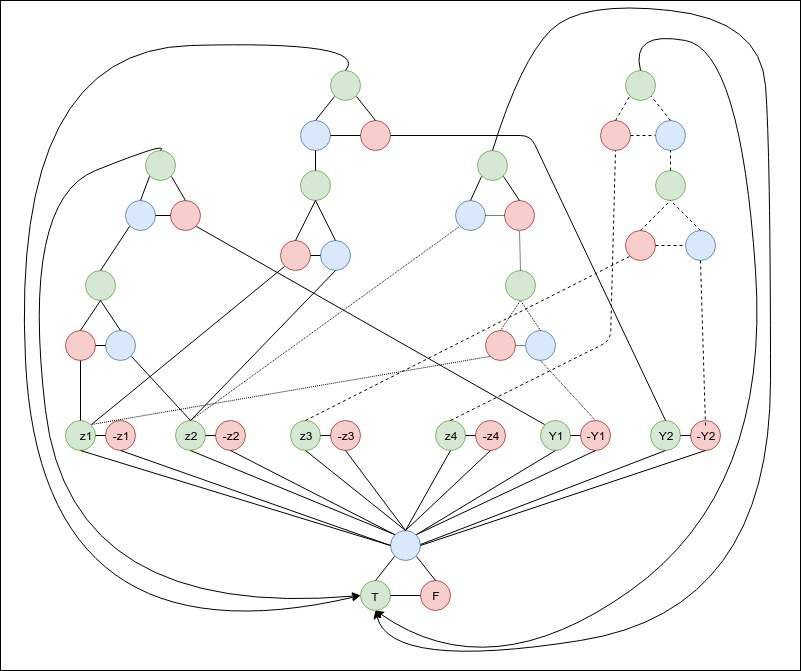
\includegraphics[width=1.0\textwidth]{images/3col.jpg}
\caption{\label{fig:3col_graph}3COL graph}
\end{figure}

\begin{equation}\label{eq:3sat-solved-formula}
F = (true \lor true \lor true) \land (false \lor true \lor true) \land (true \lor true \lor true) \land(false \lor true \lor true)
\end{equation}

Since each of the clauses of the formula evaluate to True value the complete formula also evaluates to True signifying that a valid solution has been identified for the 3SAT reduction. Furthermore it can be checked against the original problem defined in equation \ref{eq:original-problem-formula}.

Parameter substitution produces equation \ref{eq:original-formula-solved} where each of the clauses evaluates to True establishing that the whole formula can be satisfied with proposed solution.

\begin{equation}\label{eq:original-formula-solved}
F = (true \lor true) \land (true \lor true \lor true \lor true) 
\end{equation}

